\documentclass{article} %选择文档类型,我们如果是做期末大作业的话选article就可以了

\usepackage{anyfontsize}
%正如c++需要import库来实现各种各样的功能,Latex也需要调用宏包来实现各种各样的功能
\usepackage{amsmath}  %调用公式宏包
\usepackage{graphicx} %调用插图宏包
\graphicspath{{code_Latex/}}
\usepackage{ctex}     %调用中文宏包
\usepackage{float}
\usepackage{cite}


%\begin{document}这句话之前是导言区,这句话以后就开始写正文了
%可以把导言区理解为int main()函数之前的内容,而正文就是int main()主函数的部分了
\usepackage{geometry}
\geometry{left=1.5cm,right=0.5cm,top=1.0cm,bottom=1.5cm}

\begin{document}
    \title{\centerline{高性能计算实验报告}}
    \date{实验七}
    \author{信息学部 2023311704 王昕远}
    \maketitle
    \thispagestyle{empty}
% \section{top图}% \texttt{ OS版本: Linux wxy 5.15.153.1-microsoft-standard-WSL2 \#1 SMP Fri Mar 29 23:14:13 UTC 2024 x86\_64 x86\_64 x86\_64 GNU/Linux}



\section{运行截图}
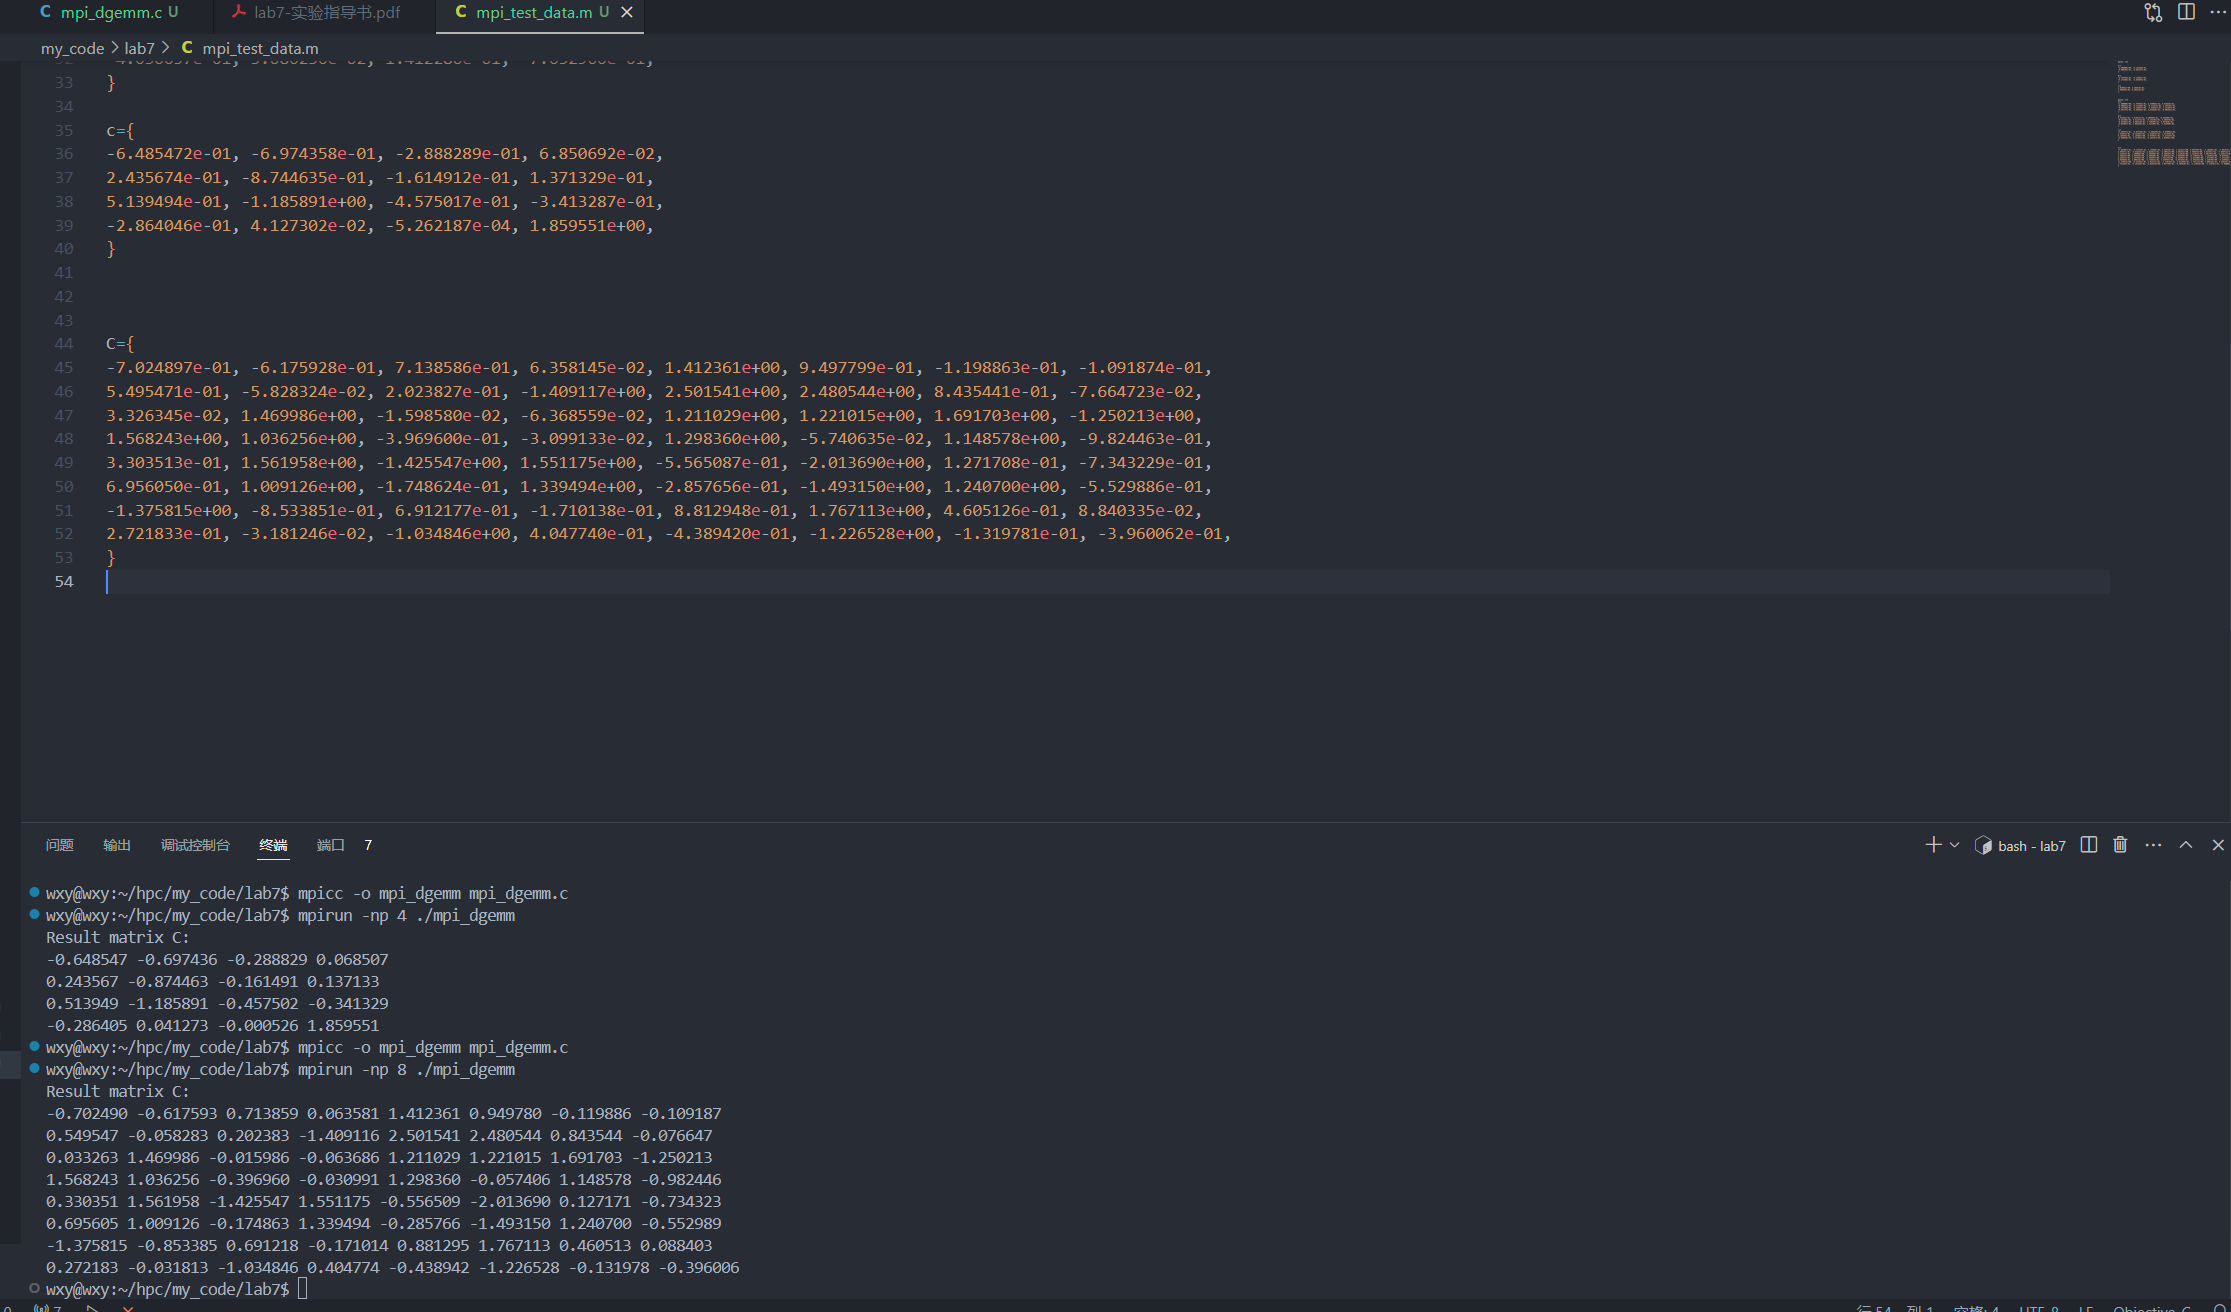
\includegraphics[width=0.8\textwidth]{i.png}






$$
$$




\end{document}